\begin{frame}{L'intégration}
    \only<1>{
    \begin{block}{Problème}
        Soit $\x(t)$ la position d’un objet rigide au temps $t$, $\v(t) =
        \dot{\x}(t)$ sa vélocité, et $\a$ son accélération constante.\\
        Trouver la position et la vélocité de l’objet au temps $t + \Delta t$.
    \end{block}
    }
    \only<2->{
    \begin{itemize}
        \item Euler explicite (instable):
            \[
                \left\{
                \begin{array}{ccl}
                    \v(t + \Delta t) & = & \v(t) + \Delta t * \a\\
                    \x(t + \Delta t) & = & \x(t) + \Delta t * \v(t)\\
                \end{array}
                \right.
            \]
            \pause
        \item Euler semi-implicite (stable):
            \[
                \left\{
                \begin{array}{ccl}
                    \v(t + \Delta t) & = & \v(t) + \Delta t * \a\\
                    \x(t + \Delta t) & = & \x(t) + \Delta t * \v(t \textcolor{red}{+ \Delta t})
                    \only<3> {
                        \\
                        \boldsymbol\omega(t + \Delta t) & = & \boldsymbol\omega(t) + \Delta t * \boldsymbol\alpha\\
                        \boldsymbol\theta(t + \Delta t) & = & \boldsymbol\theta(t) + \Delta t * \boldsymbol\omega(t \textcolor{red}{+ \Delta t})\\
                    }
                \end{array}
                \right.
            \]
    \end{itemize}
    }
\end{frame}

\begin{frame}{La détection de collision}
    \only<1> {
    \begin{block}{Problème}
        Soient $n$ objets rigides. Trouver les points et normales de contact
        entre les objets qui se touchent.
    \end{block}
    }
    \only<2> {
    \begin{figure}[h]
        \setcounter{subfigure}{0}
        \subfigure[Entrée]{
\includegraphics[height=.25\linewidth]{contact_nocontact}}
        \subfigure[Sortie]{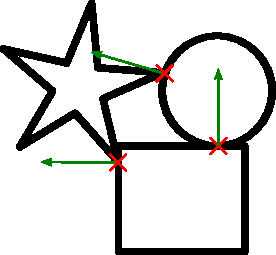
\includegraphics[height=.25\linewidth]{contact}}
    \end{figure}
    \pause
    \textbf{Il y a $n * (n - 1) / 2$ paires à tester en tout !}
    }
\end{frame}

\begin{frame}{La détection de collision}
    Que fait-on de ça ?
    \begin{center}
        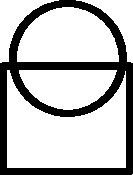
\includegraphics[scale=0.75]{penetration}
    \end{center}
    \pause
    \begin{itemize}
        \item On dit que les objets sont en \textbf{pénétration}.
            \pause
        \item La \textbf{pénétration}, c’est pas beau, et n’arrive jamais dans
            la vie réelle.
            \pause
        \item On mesure la \textbf{profondeur de pénétration}.
    \end{itemize}
    \begin{center}
        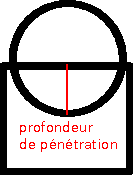
\includegraphics[scale=0.75]{penetration_depth}
    \end{center}
\end{frame}

\begin{frame}{Algorithme: boule vs. boule}
    \only<1> {
        \begin{block}{Problème}
            Soient $\A$ et $\B \subset \mathbb{R}^n$ deux boules.
            On note $r_\A$ et $r_\B \in \mathbb{R}$ leurs rayon, $\pA$et $\pB \in
            \mathbb{R}^n$ leurs position.  Calculer l’éventuelle collision.
        \end{block}
    }
    \only<2-> {
    \only<2> {
        \framesubtitle{Cas de la séparation}
        \begin{figure}[h]
            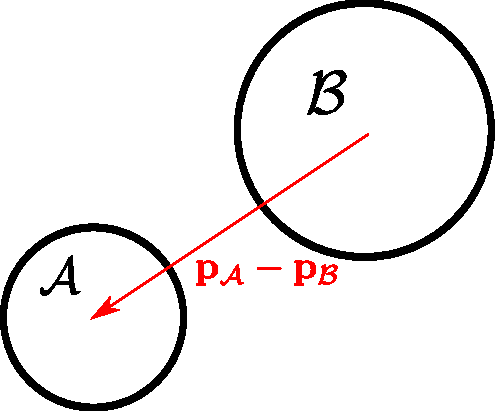
\includegraphics[height=.25\linewidth]{balls_nocollide}
        \end{figure}
        \begin{itemize}
            \item $|| \pA - \pB || > r_\A + r_\B \Rightarrow $ pas de collision.
        \end{itemize}
    }
    \only<3> {
        \framesubtitle{Cas du contact}
        \begin{figure}[h]
            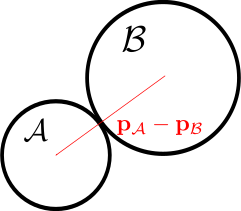
\includegraphics[height=.25\linewidth]{balls_touching}
        \end{figure}
        \begin{itemize}
            \item $|| \pA - \pB || = r_\A + r_\B \Rightarrow $ collision.
            \item normale de contact: $\n = \frac{\pA - \pB}{|| \pA - \pB ||}$.
            \item point de contact: $\pB + \n * r_\B$.
        \end{itemize}
    }
    \only<4> {
        \framesubtitle{Cas de la pénétration}
        \begin{figure}[h]
            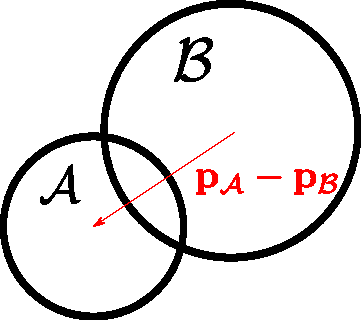
\includegraphics[height=.25\linewidth]{ball}
        \end{figure}
        \begin{itemize}
            \item $|| \pA - \pB || < r_\A + r_\B \Rightarrow $ pénétration.\\
            \item profondeur de pénétration: $r_\A + r_\B - || \pA - \pB ||$.
        \end{itemize}
    }
    }

\end{frame}

\begin{frame}[fragile]{Algorithme: objet convexe vs. plan}
    \only<1> {
    \begin{block}{Problème}
        Soit $\A$ une partie convexe de $\mathbb{R}^n$, et
        $\mathcal{P}$ un plan (demi-espace) de normale $\n$ et de position $\p$.
        Calculer l’éventuelle collision.
    \end{block}
    }
    \only<2-> {
        \only<2> {
            \framesubtitle{Notion de convexité}
                \mbox{}\\
                $\A$~convexe~$\Leftrightarrow \forall \pone, \ptwo \in \A^2, \forall \lambda \in [0, 1], \lambda *
                \pone + (1 - \lambda) * \ptwo \in \A$
                \begin{figure}[h]
                    \setcounter{subfigure}{0}
                    \subfigure[Convexe]{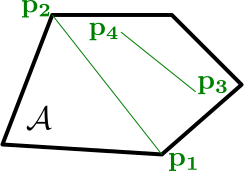
\includegraphics[height=.25\linewidth]{convexe}}
                    \subfigure[Concave]{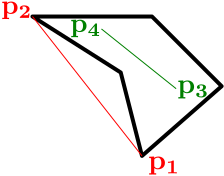
\includegraphics[height=.25\linewidth]{concave}}
                \end{figure}
        }
       \only<3> {
            \framesubtitle{Cas de la séparation}
           \begin{center}
               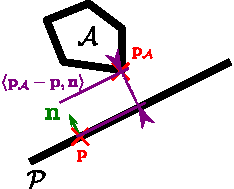
\includegraphics[height=.25\linewidth]{convex_vs_plan_nocolide}
           \end{center}
           \begin{itemize}
               \item $\left< \pA - \p, \n \right> > 0 \Rightarrow$ pas de collision.
               \item on ne sais pas (pour le moment) trouver $\pA$\ldots
           \end{itemize}
       }
       \only<4> {
            \framesubtitle{Cas du contact}
           \begin{center}
               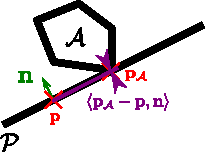
\includegraphics[height=.25\linewidth]{convex_vs_plan_contact}
           \end{center}
           \begin{itemize}
               \item $\left< \pA - \p, \n \right> = 0 \Rightarrow$ pénétration.
               \item normale de contact: $\n$.
               \item point de contact: $\pA$.
           \end{itemize}
       }
       \only<5> {
            \framesubtitle{Cas de la pénétration}
           \begin{center}
               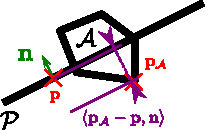
\includegraphics[height=.25\linewidth]{convex_vs_plan_penetration}
           \end{center}
           \begin{itemize}
               \item $\left< \pA - \p, \n \right> < 0 \Rightarrow$ pénétration.
               \item Profondeur de pénétration: $\left< \pA - \p, \n\right>$.
           \end{itemize}
       }
   %\begin{description}
       %\item
        \only<6,7> {
            \framesubtitle{Déterminer $\pA = s_\A(-\n)$}
        %\item[Fonction de support:]\mbox{}\\
                \begin{itemize}
                    \item On définit la \textbf{fonction de support} $s_\A(\v)$
                        de $\A$:
                        \[
                            s_\A(\v) = \argmax\limits_{\p \in \A} \left< \p, \v \right>
                        \]
                \end{itemize}
                \visible<7> {
                    \begin{center}
                        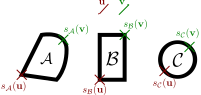
\includegraphics[height=.25\linewidth]{support_fun}
                    \end{center}
                }
        }
        \only<8> {
            \framesubtitle{Algorithme final}
            \begin{algorithm}[H]
            \begin{algorithmic}[1]
                \STATE $\pA  = s_\A(-\n)$
                \STATE $d = \left< \pA - \p, \n \right>$
                \IF{$d > 0$}
                    \RETURN Pas de collision.
                \ENDIF
                \RETURN (normale: $\n$, point: $\pA - \n * d$, pénétration: $d$)
            \end{algorithmic}
            \end{algorithm}
                \begin{center}
                    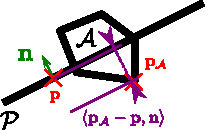
\includegraphics[height=.15\linewidth]{convex_vs_plan_penetration}
                \end{center}
        }
    }
    %\end{description}
\end{frame}

\begin{frame}{Théorie: objet convexe vs. objet convexe}
    \only<1> {
    \begin{block}{Problème}
        Soient $\A$ et $\B$ deux parties convexes de
        $\mathbb{R}^n$, trouver $\pii \in \A$ et $\pj \in
        \B$, tels que $|| \pii - \pj || = 0$.
    \end{block}
    }
    \only<2-> {
        \framesubtitle{La somme de Minkowski}
    \only<2-4> {
    \begin{itemize}
        \item<2-4> Soit $\A \oplus -\B = \{ \pii + (-\pj) \mid \pii \in
            \A \text{ et } \pj \in \B \}$\\
            Deux objets sont en collision ssi $0_{\mathbb{R}^n} \in
            \A \oplus -\B$.
        \item<3-4> Les points les plus proches entre $\A$ et
            $\B$ sont donnés par: \[ \argmin\limits_{\pii \in
            \A, \pj \in \B} || \pii - \pj || \]
        \item<4> La plus petite distance est donnée par:
            \[ \min\limits_{\pii \in \A,
            \pj \in \B} || \pii - \pj || \]
            C’est la distance entre $\A \oplus -\B$ et l’origine~!
    \end{itemize}
    }
    \only<5> {
        \begin{center}
            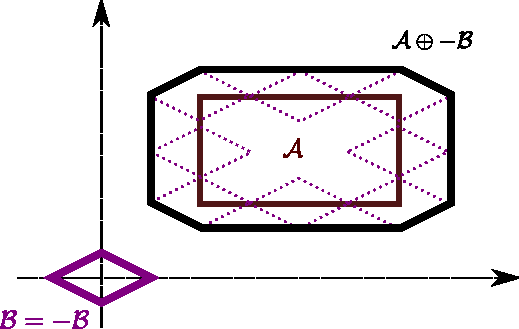
\includegraphics[scale=0.9]{a_plus_minus_b}
        \end{center}
    }
    \only<6> {
        \begin{center}
            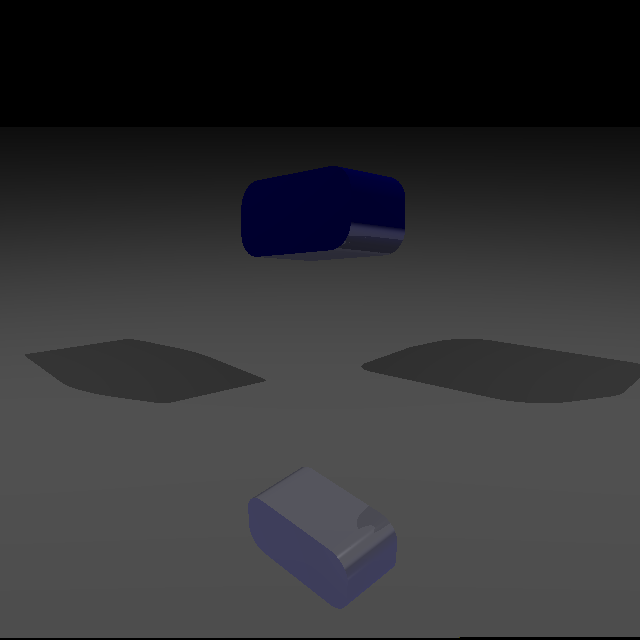
\includegraphics[scale=0.25]{box_plus_cylinder}\\
            Boite $\oplus$ Cylindre
        \end{center}
    }
    \only<7-> {
    \begin{itemize}
        \item<7-> $\A \oplus \B$ est la \textbf{Somme de Minkowski} de $\A$ et $\B$.
        \item<8-> $\A \oplus - \B$ est le \textbf{Configuration Space Obstacle} (CSO).
        \item<9-> Le CSO est très lourd à calculer explicitement.
        \item<10-> Mais sa fonction de support est facile à évaluer:
            \[
                s_{\A \oplus - \B}(\v) = s_\A(\v) - s_\B(-\v)
            \]
    \end{itemize}
    }
    }
\end{frame}

\begin{frame}{Algorithme: objet convexe vs. objet convexe}
    \only<1> {
        \framesubtitle{L’algorithme de Gilbert–Johnson–Keerthi (GJK)}
        \begin{itemize}
            \item Le GJK calcule la distance entre l’origine et un ensemble convexe.
            \item Utilise uniquement la fonction de support de l’ensemble.
            \item Peut être utilisé sur le CSO pour détecter une collision.
        \end{itemize}
    }
    \only<2-5> {
        \framesubtitle{L’algorithme de Gilbert–Johnson–Keerthi (GJK): cas de la séparation.}
    }
    \only<2> {
        \centering
        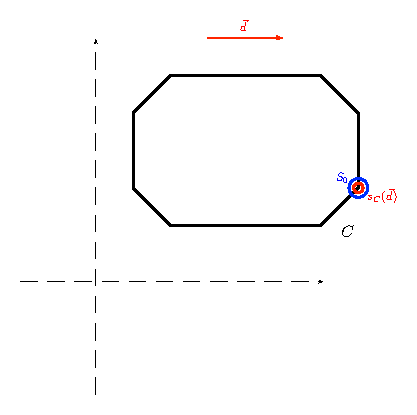
\includegraphics{minkowski_gjk_01}
    }
    \only<3> {
        \centering
        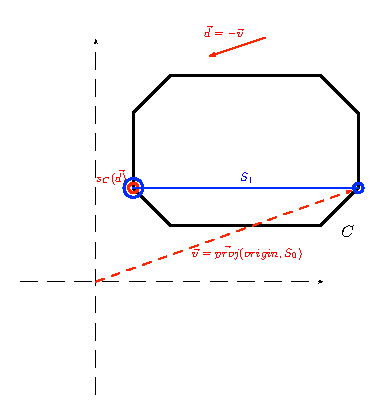
\includegraphics{minkowski_gjk_02}
    }
    \only<4> {
        \centering
        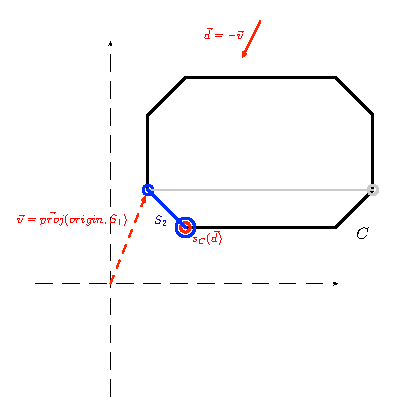
\includegraphics{minkowski_gjk_03}
    }
    \only<5> {
        \centering
        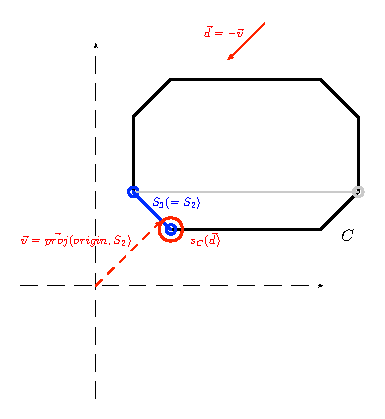
\includegraphics{minkowski_gjk_04}
    }
    \only<6> {
        \begin{itemize}
            \item Ne fonctionne \textbf{pas} si l’origine est à l’intérieur de
                l’objet!
            \item Or, l’origine est à l’intérieur du CSO si les objets sont en
                collision…
            \item Il faut donc utiliser un autre algorithme pour calculer les
                détails d’une collision.
        \end{itemize}
    }
    \only<7-9> {
        \framesubtitle{L’algorithme de Gilbert–Johnson–Keerthi (GJK): cas de la pénétration.}
    }
    \only<7> {
        \centering
        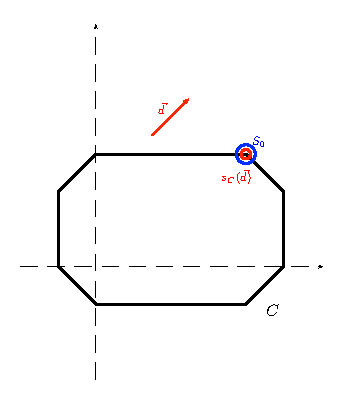
\includegraphics{minkowski_gjk_11}
    }
    \only<8> {
        \centering
        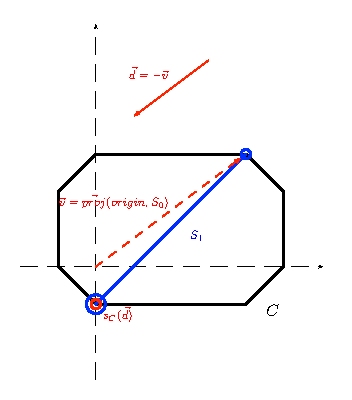
\includegraphics{minkowski_gjk_12}
    }
    \only<9> {
        \centering
        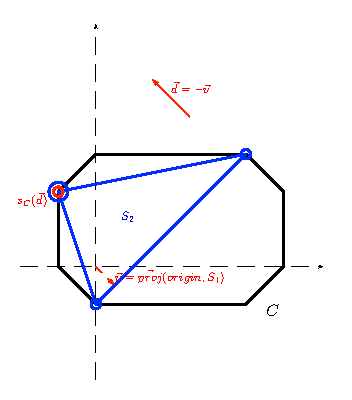
\includegraphics{minkowski_gjk_13}
    }
    \only<10-> {
        \framesubtitle{Échantillonage du CSO.}
    }
    \only<10> {
        \begin{itemize}
            \item Le GJK ne fonctionne pas pour calculer les pénétrations.
            \item Un autre algorithme peut prendre la main.
            \item Échantilloner le CSO donne une bonne approximation.
        \end{itemize}
    }
    \only<11> {
        \centering
        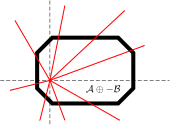
\includegraphics[scale=1.75]{sampling_noproj}
    }
    \only<12> {
        \centering
        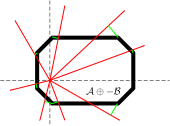
\includegraphics[scale=1.75]{sampling_proj}
    }
    \only<13> {
        \centering
        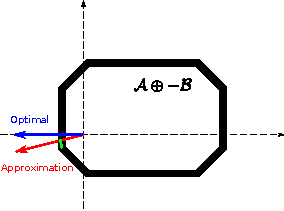
\includegraphics[scale=1.75]{sampling_bestproj}
    }
\end{frame}

\begin{frame}{Détection impliquant des objets concaves}
    \pause
    \begin{enumerate}
        \item Décomposer en parties convexes (une fois pour toutes).
        \item Calculer les collisions entre parties convexes.
    \end{enumerate}
    \begin{center}
        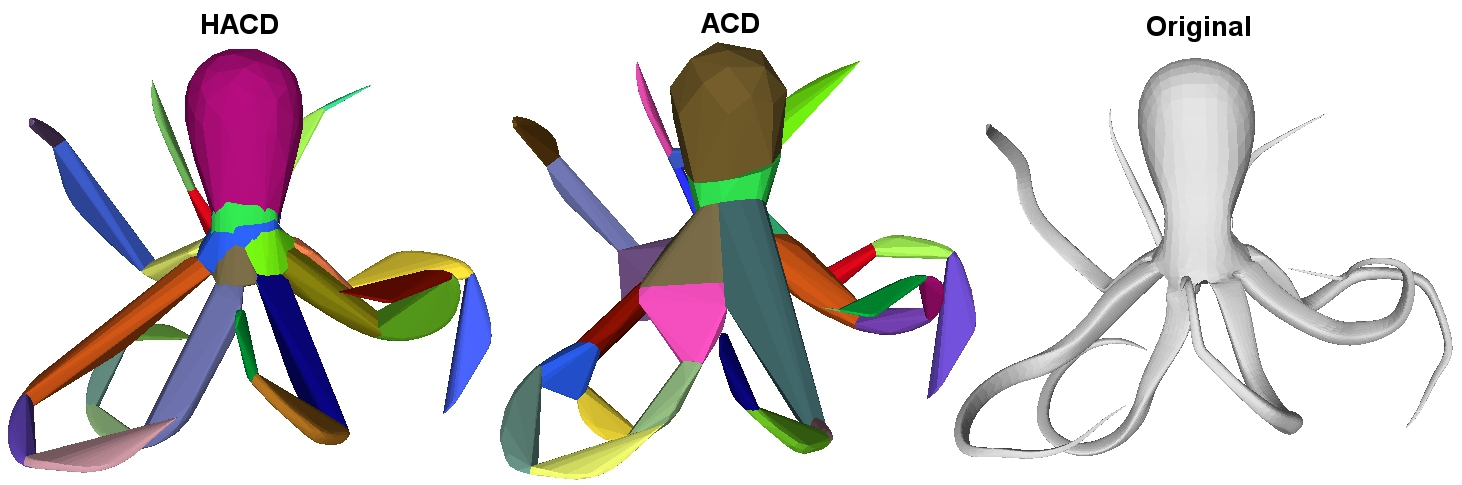
\includegraphics[height=.25\linewidth]{decomp_3d}\\
        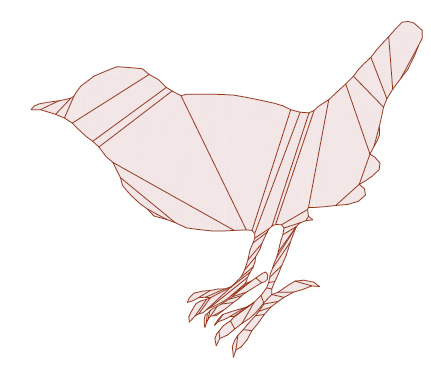
\includegraphics[height=.25\linewidth]{decomp_2d}
    \end{center}
\end{frame}

\begin{frame}{Le calcul des forces de contact}
    \begin{block}{Problème}
         Soit un ensemble de $n$ contacts $C_i, i \in [1, n]$. Quelles sont les
         forces à appliquer aux objets afin qu’ils réagissent de manière
         réaliste?
    \end{block}
    \pause
    Il \textit{suffit} de résoudre une (M)LCP:
    \[
    \left\{
        \begin{array}{l}
            JM^{-1}J^T {\color{red}{\lambda}} = \zeta +
            J(V^1 - M^{-1}F * \Delta t)\\
            0 \leq {\color{red}{\lambda}} \leq +\infty % +\infty
        \end{array}
    \right.
    \]
    \begin{center}
        
\includegraphics[height=.25\linewidth]{scared_cat}
    \end{center}
\end{frame}

\begin{frame}{Le calcul des forces de contact}
    \begin{block}{Charactéristiques d’un objet rigide $\mathcal{R}_i$}
    \begin{itemize}
        \item Centre de gravité: $\cofmass_i$
        \item Masse:             $m_i$
        \item Tenseur d’inertie: $I_i$
        \item Vélocité linéaire: $\v_i$
        \item Vélocité angulaire: $\w_i$
        \item Forces subies: $\f_i$
        \item Moments subis: $\btau_i$
    \end{itemize}
    \end{block}

    \pause

    \begin{block}{Charactéristiques d’un contact $C$}
    \begin{itemize}
        \item Point de contact: $\cofmass$
        \item Profondeur de pénétration: $d$
        \item Normale de contact: $\n$
    \end{itemize}
    \end{block}
\end{frame}

\begin{frame}{Le calcul des forces de contact}
    \framesubtitle{Équations de mouvement}
    Équations de mouvement pour $\mathcal{R}_i$:\\
    \begin{center}
    \begin{math}
        \begin{array}{lcl}
            \sum \f_i & = & m_i\a_i \\[0.5em]
            \pause
            \sum \f_i & = & m_i \frac{\v_i^{t + \Delta t} - \v_i^t}{\Delta t} \\[0.5em]
            \pause
            \Delta t * m_i^{-1} * \sum \f_i & = & \v_i^{t + \Delta t} - \v_i^t
        \end{array}
    \end{math}
    \end{center}

    \pause
    On obtient simplement un intégrateur d’Euler:
    \begin{center}
    \cfbox{red}{
        $\v_i^{t + \Delta t} = \v_i^t + \Delta t * m_i^{-1} * \sum \f_i$
    }
    \end{center}
    \pause
    Le même chose pour les rotations:
    \begin{center}
    \cfbox{red}{
        $\bomega_i^{t + \Delta t} = \bomega_i^t + \Delta t * I_i^{-1} * \sum \btau_i$
    }
    \end{center}
\end{frame}

\begin{frame}{Le calcul des forces de contact}
    \framesubtitle{Équations de mouvement}
    Il est possible de regrouper les deux équations en une seule avec:
    \[
        V_i = \left[ \begin{array}{c} \v_i\\\bomega_i\end{array}\right]
        M_i = \left[ \begin{array}{c} m_i\\I_i\end{array}\right]
        F_i = \left[ \begin{array}{c} \sum \f_i\\\sum \btau_i\end{array}\right]
    \]
    \pause
    \begin{center}
    \cfbox{red}{
        $V_i^{t + \Delta t} = V_i^t + \Delta t * M_i^{-1} * F_i$
    }
    \end{center}
\end{frame}

\begin{frame}{Le calcul des forces de contact}
    \framesubtitle{Contrainte de contact}
    L’effet d’un contact parfaitement inélastique est de supprimer toute
    vélocité relative selon la normale de contact.
    \begin{description}
        \item[Vélocité relative:]
    \end{description}
    \pause
    \begin{center}
        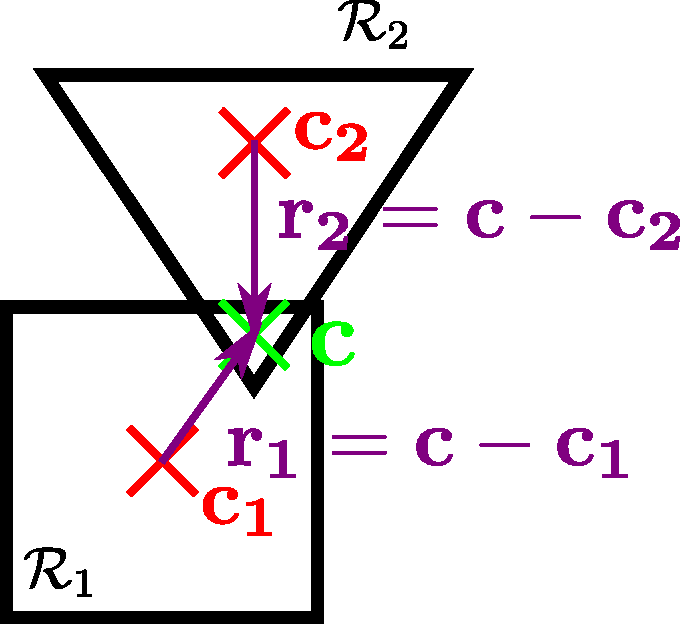
\includegraphics[scale=0.25]{coll_conf}
    \end{center}
    \pause
    \begin{itemize}
        \item Contribution linéaire:
            $
                \left< \n, \v_1^{t + \Delta t} \right> -
                \left< \n, \v_2^{t + \Delta t} \right>
            $
            \pause
        \item Contribution rotationelle:
            $
                \left<\r_1 \times \n, \bomega_1^{t + \Delta t} \right> -
                \left<\r_2 \times \n, \bomega_2^{t + \Delta t} \right>
            $
    \end{itemize}
\end{frame}

\begin{frame}{Le calcul des forces de contact}
    \framesubtitle{Contrainte de contact}
    \begin{description}
        \item[Contrainte résultante:]
    \end{description}
    \begin{math}
        \left< \n, \v_1^{t + \Delta t} \right> -
        \left< \n, \v_2^{t + \Delta t} \right> +
        \left<\r_1 \times \n, \bomega_1^{t + \Delta t} \right> -
        \left<\r_2 \times \n, \bomega_2^{t + \Delta t} \right>
        = 0
    \end{math}
    \pause
    \mbox{}\\[1em]
    \begin{math}
        \left< \n, \v_1^{t + \Delta t} \right> +
        \left<\r_1 \times \n, \bomega_1^{t + \Delta t} \right> -
        \left< \n, \v_2^{t + \Delta t} \right> -
        \left<\r_2 \times \n, \bomega_2^{t + \Delta t} \right>
        = 0
    \end{math}
    \pause
    \mbox{}\\[1em]
    \begin{math}
        {
            \color{blue}
        \left[
            \n^T               \hspace{0.75em}
            (\r_1 \times \n)^T \hspace{0.75em}
            -\n^T              \hspace{0.75em}
            -(\r_2 \times \n)^T
        \right]
        }
        {
            \color{brown}
        \left[
            \begin{array}{c}
            \v_1^{t + \Delta t}      \\
            \bomega_1^{t + \Delta t} \\
            \v_2^{t + \Delta t}      \\
            \bomega_2^{t + \Delta t}
            \end{array}
        \right]
        }
        = 0
    \end{math}
    \pause
    \mbox{}\\[1em]
    \begin{center}
        \cfbox{red}{
            ${\color{blue}J} * {\color{brown}V^{t + \Delta t}} = 0$
        }
    \end{center}
\end{frame}

\begin{frame}{Le calcul des forces de contact}
    On a donc:
    \[
        \left\{
        \begin{array}{lcl}
            J * \color{red}V^{t + \Delta t} & = & 0\\
            \color{red}V^{t + \Delta t}     & = & V^t + \Delta t * M^{-1} * F
        \end{array}
        \right.
    \]
    \pause
    D’où:
    \[
        \begin{array}{lcl}
            J ({\color{red}V^t + \Delta t * M^{-1} * F}) & = & 0\\
            \pause
            J (V^t + \Delta t * M^{-1} * (F_{\text{ext}} +
            F_{\text{contacts}})) & = & 0\\
            \pause
            -J(V^t + \Delta t * M^{-1} * F_{\text{ext}}) & = &  \Delta t * J * M^{-1} * F_{\text{contacts}}\\
        \end{array}
    \]
    \pause
    Les forces de contact sont supportées par les normales et les axes de
    rotation instantanés donc: $\Delta t * F_{\text{contacts}} = J^T * \lambda$ avec
    $\frac{\lambda}{\Delta t}$ l’intensité des forces:
    \pause
    \begin{center}
    \cfbox{red}{
        $-J(V^t + \Delta t M^{-1} F_{\text{ext}}) = J M^{-1} J^T \lambda$
    }
    \end{center}
\end{frame}

\begin{frame}{Le calcul des forces de contact}
    \begin{itemize}
        \item Pour corriger les pénétrations, on ajoute de l’énergie au système
            égal à $\zeta$, proportionnel à la profondeur de pénétration:
            \begin{center}
            \cfbox{red}{
                $\zeta - J(V^t + \Delta t M^{-1} F_{\text{ext}}) = J M^{-1} J^T \lambda$
            }
            \end{center}
            \pause
        \item La MLCP peut être résolue avec l’algorithme de Gauss-Seidel
            Projeté.
            \pause
        \item Des méthodes directes existent, mais nécessitent un algorithme de
            fallback.
    \end{itemize}
\end{frame}
